\documentclass{article}

% Set page size and margins
\usepackage[a4paper,top=2cm,bottom=2cm,left=2.5cm,right=2.5cm,marginparwidth=1.75cm]{geometry}

% Useful packages

\usepackage{graphicx}
%\usepackage[draft]{graphicx}

\usepackage{amsmath}
\usepackage{wrapfig}
\usepackage{subcaption}
\usepackage{caption}
\usepackage{float}
\usepackage{multicol}
\usepackage[colorlinks=true, allcolors=blue]{hyperref}
\usepackage{lscape} 
\usepackage{authblk}

\renewcommand\arraystretch{1.25}

\usepackage{listings}
\usepackage{color}
\usepackage[percent]{overpic}

\definecolor{dkgreen}{rgb}{0,0.6,0}
\definecolor{gray}{rgb}{0.5,0.5,0.5}
\definecolor{mauve}{rgb}{0.58,0,0.82}

\lstset{frame=tb,
  language=R,
  aboveskip=3mm,
  belowskip=3mm,
  showstringspaces=false,
  columns=flexible,
  basicstyle={\small\ttfamily},
  numbers=none,
  numberstyle=\tiny\color{gray},
  keywordstyle=\color{blue},
  commentstyle=\color{dkgreen},
  stringstyle=\color{mauve},
  breaklines=true,
  breakatwhitespace=true,
  tabsize=3
}

\counterwithout*{figure}{section} % this is the only way i got the figure number and in-text reference to match, no idea what kind of black magic is happening here though


\title{TODO title about Y-haplotype effect on larval transcriptome}
\author[1]{Milena Trabert}
\author[1]{Bianca Sarcani}
\author[2]{Philipp Kaufmann}
\author[1]{Elina Immonen}
\date{ }
\affil[1]{Department of Ecology and Genetics (Evolutionary Biology program), Evolutionary Biology Centre, Norbyvägen 18D, 75236, Uppsala University, Uppsala}
\affil[2]{Philipp's current affiliation}

\begin{document}
\pagenumbering{gobble}
\maketitle
\newpage
\renewcommand{\arraystretch}{1.5}
\renewcommand{\thetable}{S\arabic{table}}
\renewcommand{\thefigure}{S\arabic{figure}}

% pdflatex -pdf supplementary_information.tex


\begin{figure}[H]

    \begin{subfigure}[t]{0.49\linewidth}
	    \begin{picture}(0,0)
   	  		\put(22,-15){\textbf{A}} % adjust the x and y values here
		\end{picture}
	    \begin{center}
        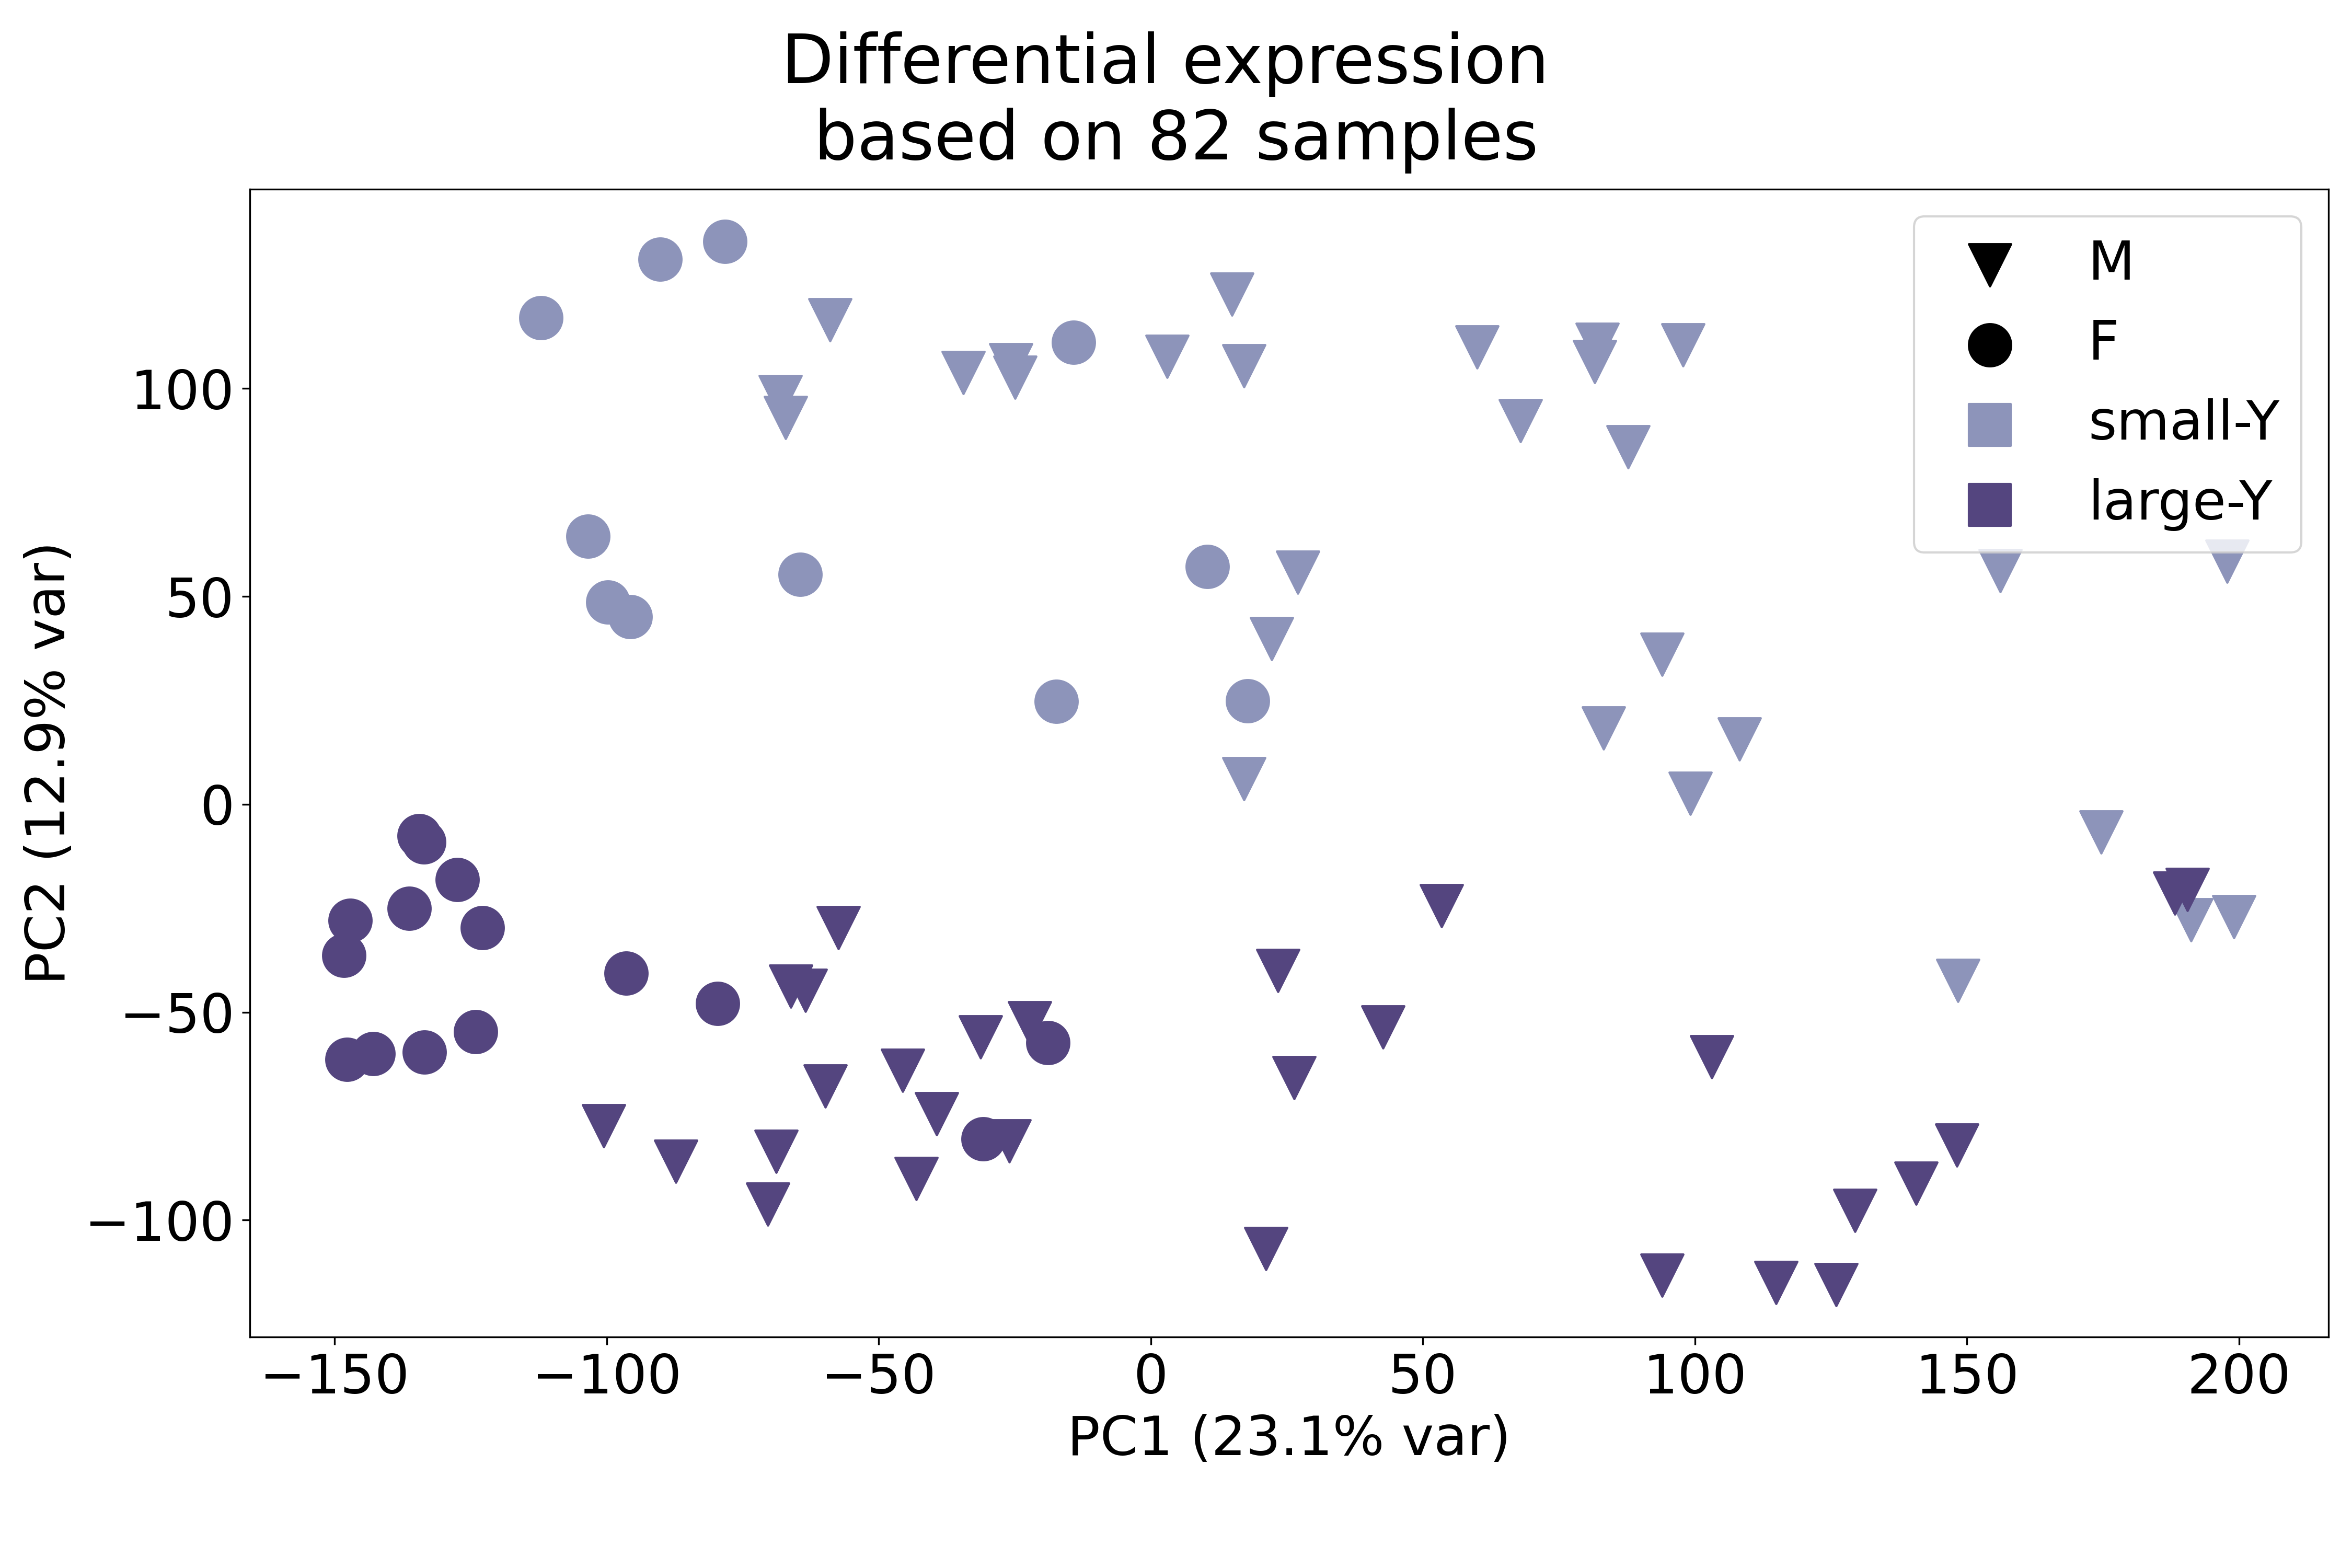
\includegraphics[width=\linewidth]{../data/DE_figures/PCA_sex_line_all_counts.png}
        \end{center}        
    \end{subfigure}
    \begin{subfigure}[t]{0.49\linewidth}
        \begin{picture}(0,0)
            \put(22,-15){\textbf{B}} % adjust the x and y values here
		\end{picture}
        \begin{center}
        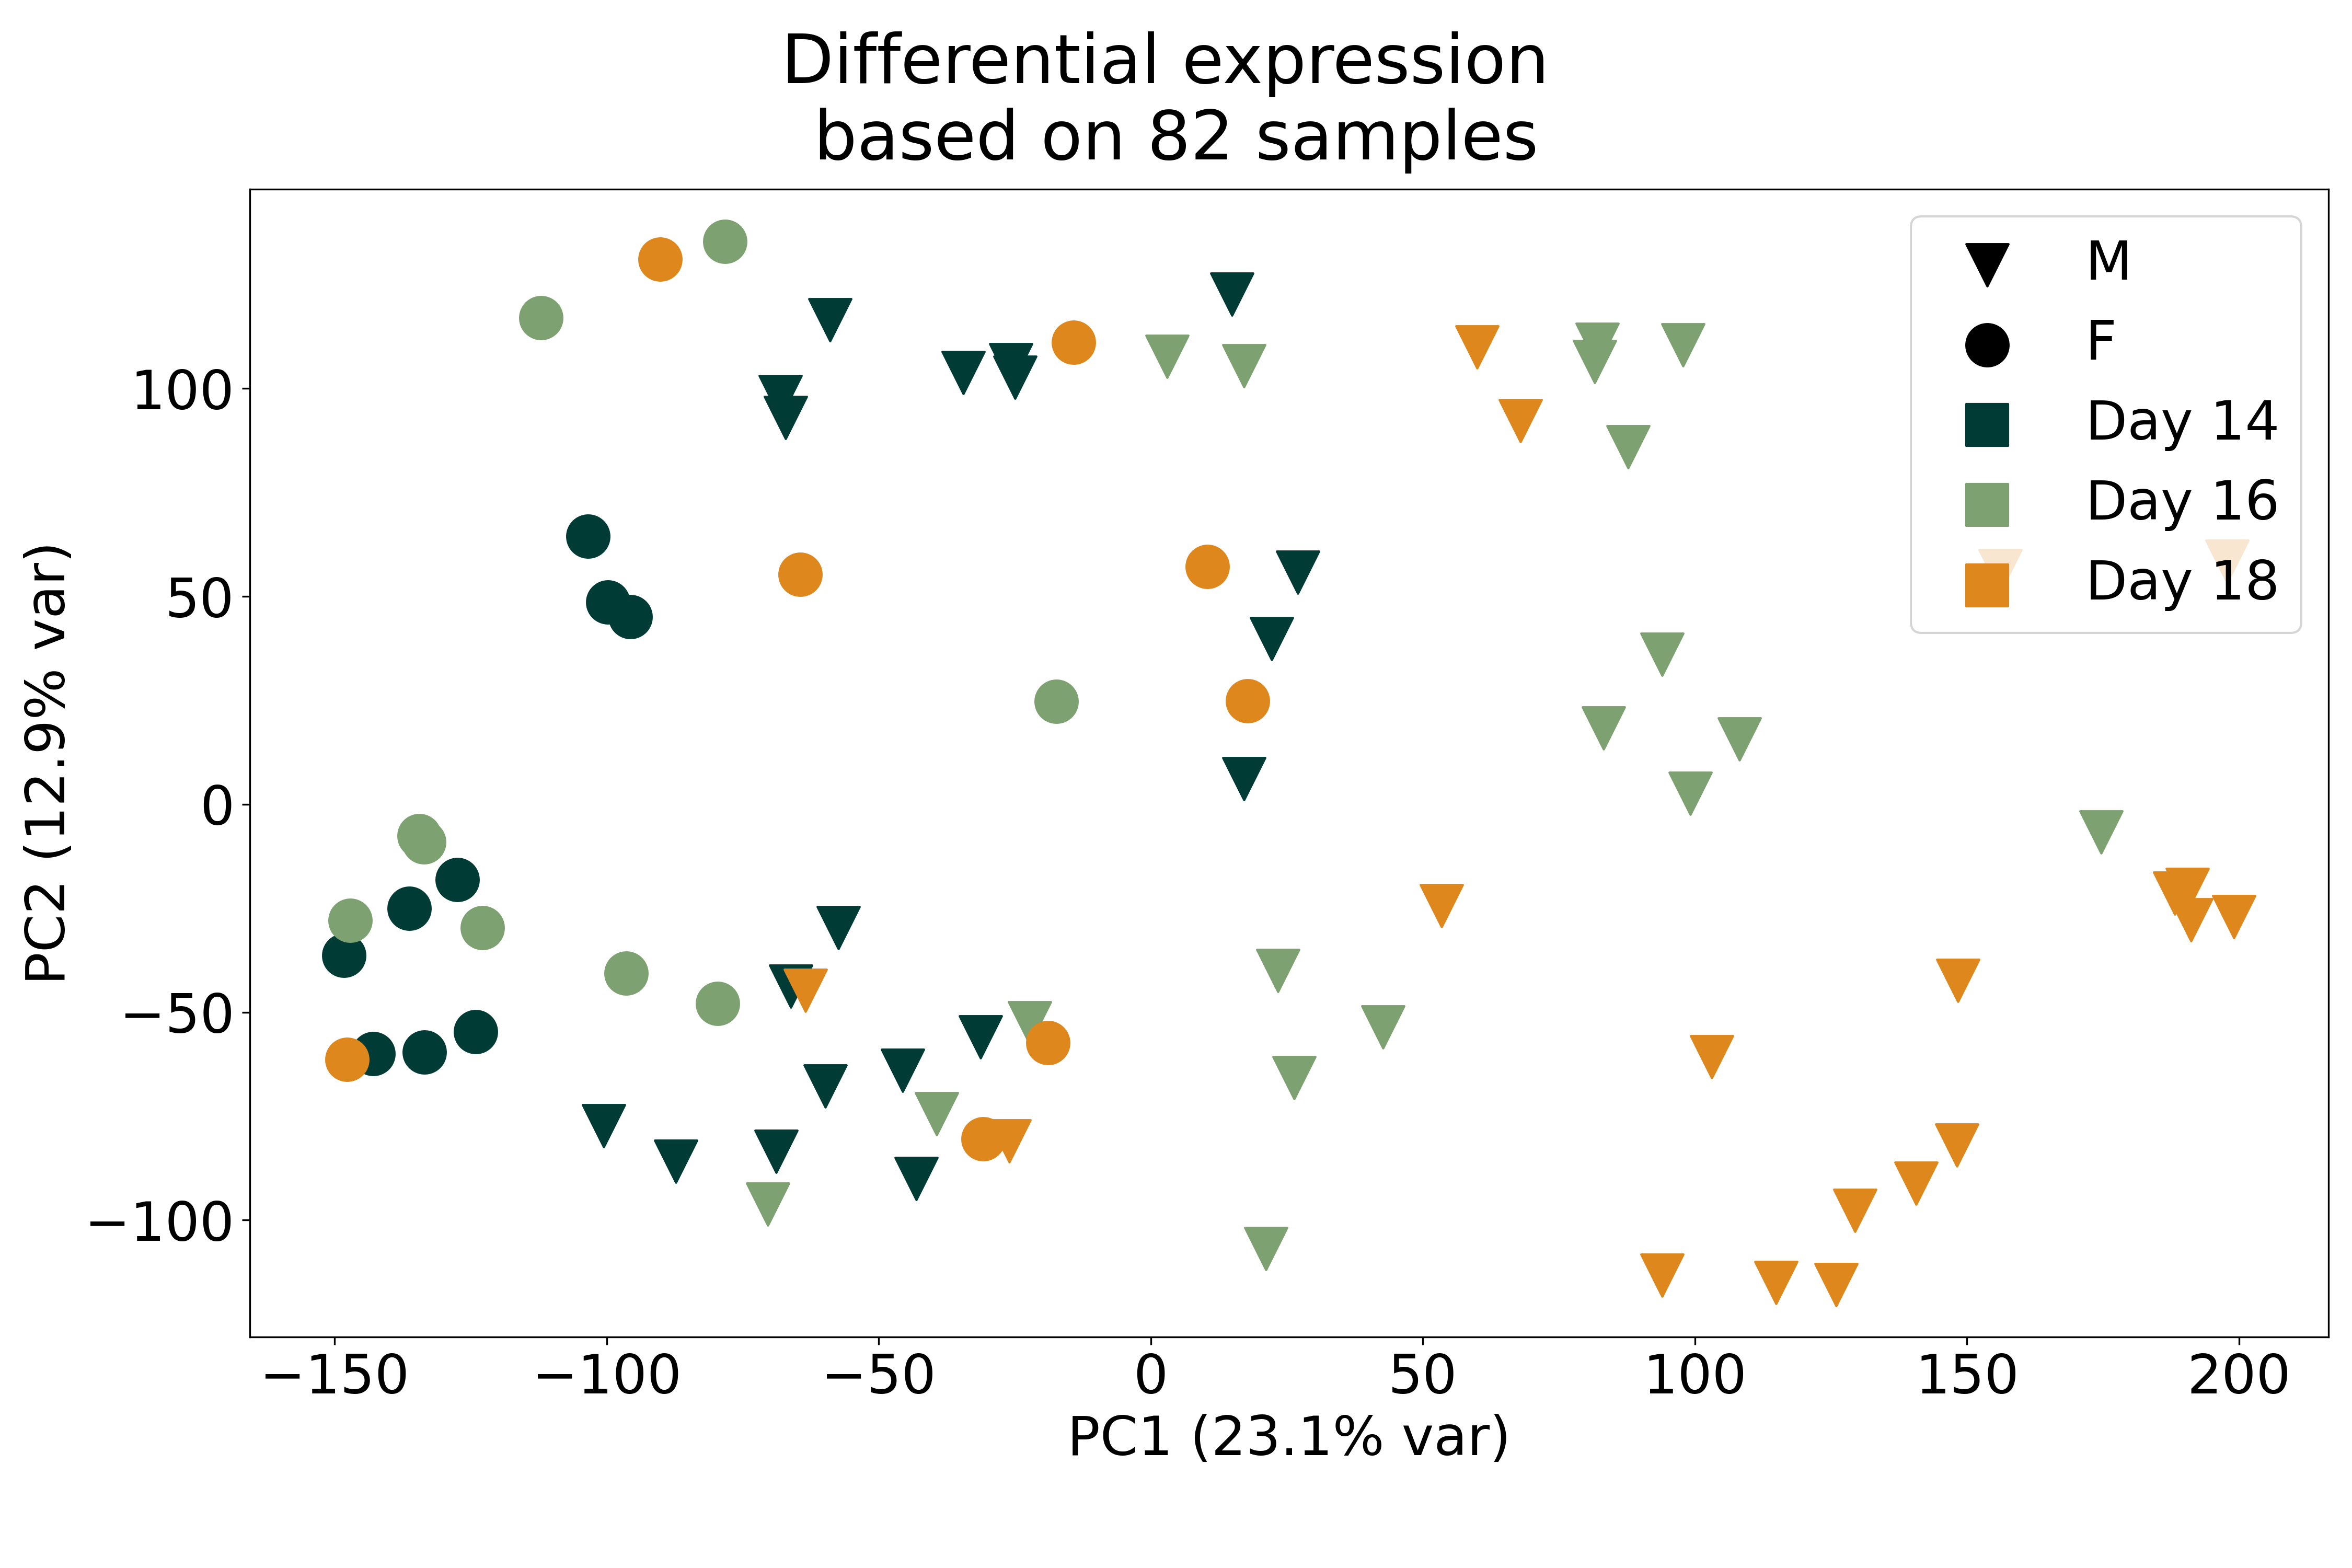
\includegraphics[width=\linewidth]{../data/DE_figures/PCA_sex_day_all_counts.png}
        \end{center}        
    \end{subfigure}
    
    \caption{\textbf{Line-biased genes in males}. 
    (\textbf{A}, \textbf{B}) PCA of all samples, hightlighted by Y-haplotype (A) or time point (B).
    }\label{day_split}
    
\end{figure}



\end{document}